\documentclass{article}

\usepackage[final]{neurips_2026}

\usepackage[utf8]{inputenc}
\usepackage[T1]{fontenc}
\usepackage{hyperref}
\usepackage{url}
\usepackage{booktabs}
\usepackage{amsfonts}
\usepackage{amsmath}
\usepackage{amssymb}
\usepackage{amsthm}
\usepackage{nicefrac}
\usepackage{microtype}
\usepackage{xcolor}
\usepackage{graphicx}
\usepackage{subcaption}
\usepackage{multirow}
\usepackage{tikz}
\usetikzlibrary{positioning,arrows.meta}

\newtheorem{theorem}{Theorem}
\newtheorem{proposition}{Proposition}
\newtheorem{definition}{Definition}
\newtheorem{remark}{Remark}

\title{Physiology-Constrained Learning: Noisy Physiological\\Consistency Constraints for Cross-Hospital Generalization}

\author{%
  Nikhil Tamvada
}

\begin{document}
\raggedbottom

\maketitle

\begin{center}
\emph{In-progress research draft --- not for distribution.}
\end{center}

\begin{abstract}
Clinical AI models degrade under cross-hospital deployment because they encode
site-specific measurement artifacts rather than universal physiological mechanisms.
We observe that known algebraic relationships---governing blood pressure, acid-base
balance, and oxygen dissociation---are approximately conserved across hospitals up to
bounded measurement noise, providing a label-free consistency signal in the spirit of
the Independent Causal Mechanisms principle without requiring environment labels.
We introduce Physiology-Constrained Learning (PCL), which augments masked
prediction pretraining with differentiable penalties that softly enforce consistency
with these physiological relationships among predicted variables, encouraging
representations that encode physiological structure rather than site-specific
correlations.
A 3.2M-parameter transformer trained on PhysioNet Challenge 2019 Site~A for
sepsis onset prediction (Sepsis-3) achieves zero-shot transfer to three held-out
cohorts---Site~B and the full-scale MIMIC-IV ($\sim$73k stays) and eICU
($\sim$200k stays, 186 hospitals) databases---spanning two independent EHR systems
without any target-domain data.
PCL improves out-of-distribution sepsis AUROC over ERM at every held-out site---by
$8.6$ points on the geographically diverse eICU benchmark, $9.7$ on MIMIC-IV, and
$6.5$ on same-system mild shift (Site~B)---while also improving in-distribution
($+3.9$). IRM provably fails in the low-environment regime~(Rosenfeld et al.\ 2021),
confirmed here with $k{=}3$ care-unit environments ($-2.3$pp vs.\ ERM), and standard
DRO does not exceed ERM under limited group supervision.
Linear probe analysis reveals that PCL substantially enriches clinically relevant
representations while hospital site discriminability remains
equivalent for both models, indicating that physiological
constraints enrich universal clinical feature encoding rather than suppress site
information.
A constraint randomization ablation---testing incorrect, shuffled, and noise-injected
variants alongside real equations---confirms that physiological correctness, not
generic regularization, is the primary driver of OOD gains.
The PCL violation score additionally functions as a calibration-free OOD detector.
\end{abstract}

%=============================================================================
\section{Introduction}
\label{sec:intro}
%=============================================================================

In March 2020, the University of Michigan Hospital deactivated its AI sepsis alert system after COVID-19 patients triggered a surge of spurious alarms~\citep{wong2021external}.
The model had learned local statistical patterns---not the physiology of sepsis.
This failure is not anomalous: clinical AI models trained at one hospital degrade systematically when deployed at another~\citep{zech2018variable, futoma2020myth, nestor2019feature}, and the FDA, WHO, and major hospital systems identify cross-hospital generalization as the primary barrier to real-world deployment~\citep{fda2021action}.

The root cause is that models learn hospital-specific shortcuts: different blood pressure cuff brands produce systematically biased MAP readings, local lab analyzer calibrations shift pH and electrolyte values, and institutional ordering habits create spurious correlations between measurement timing and outcomes~\citep{finlayson2021clinician}.
Standard remedies---domain adaptation~\citep{ganin2016domain}, federated learning~\citep{rieke2020future}, and data augmentation---either require target domain data (unavailable at deployment) or operate at the input level without constraining what the representation encodes.

Invariant Risk Minimization (IRM)~\citep{arjovsky2019invariant} enforces invariance across environments, but Rosenfeld et al.~\citep{rosenfeld2021risks} formally proved IRM fails when the number of environments $k$ is small relative to the dimensionality of spurious features.
In clinical settings, $k < 10$ source hospitals is typical, placing IRM firmly in its failure regime.

We propose a different invariance signal: \emph{approximate physiological consistency constraints}.
The algebraic relationships linking clinical variables are approximately conserved across hospitals, even though local measurement devices and calibration procedures vary.
Mean arterial pressure closely tracks $\text{DBP} + \nicefrac{1}{3}(\text{SBP} - \text{DBP})$.
pH approximately obeys Henderson-Hasselbalch.
These relationships carry no hospital index beyond bounded sensor noise, motivating them as a label-free invariance signal in the spirit of the Independent Causal Mechanisms (ICM) principle~\citep{scholkopf2021toward}, under which causal mechanisms are modular and largely environment-independent.

\textbf{Physiology-Constrained Learning (PCL)} operationalizes this insight as a differentiable pretraining objective.
We add soft penalties for physiological consistency violations to the standard masked prediction loss, encouraging the model's internal representation to encode the algebraic structure of the domain rather than hospital-specific biases.
Critically, PCL requires no environment labels ($k = 0$), no target domain data, and no architectural modification---only the domain equations themselves.

\paragraph{Contributions.}
\textbf{(1) PCL as a physiological-consistency pretraining strategy}: differentiable physiological penalties produce site-robust representations enabling zero-shot cross-hospital transfer, with gains at every held-out site and the largest on high-diversity OOD benchmarks (eICU: $+8.6$pp, MIMIC-IV: $+9.7$pp over ERM; Section~\ref{sec:method}).
\textbf{(2) IRM failure in the clinical low-environment regime}: IRM with $k{=}3$ environments degrades below ERM while PCL requires no environment labels, validating Rosenfeld et al.; standard DRO likewise fails to exceed ERM under limited group supervision.
\textbf{(3) PCL violation as a calibration-free OOD detector}: no labeled OOD data, no extra parameters (Section~\ref{sec:ood_detector}).

%=============================================================================
\section{Related Work}
\label{sec:related}
%=============================================================================

PCL departs from environment-based invariance methods---most directly IRM~\citep{arjovsky2019invariant}, which provably degrades when the number of environments is small~\citep{rosenfeld2021risks}, and worst-group DRO~\citep{sagawa2020distributionally}---by encoding the causal structure of the domain directly rather than treating environments as a proxy for it. It is likewise distinct from recent ICU foundation models, which use standard masked or autoregressive pretraining objectives without physiological constraints~\citep{icarefm2025}, and from physics-informed neural networks~\citep{raissi2019physics}, which enforce physical laws for simulation accuracy rather than for distribution-invariant representations.

%=============================================================================
\section{Method}
\label{sec:method}
%=============================================================================

\subsection{Problem Formulation}

Let $\mathcal{X} = \{x^{(i)}\}_{i=1}^N$ denote multivariate clinical time series from a source hospital, where $x^{(i)} \in \mathbb{R}^{T \times V}$ represents $V$ clinical variables observed over $T$ hourly timesteps.
We seek a representation $z = f_\theta(x)$ such that a downstream classifier $g_\phi(z)$ achieves strong performance not only on the source distribution but also on data from unseen hospitals---without access to any target domain data during training.

\begin{definition}[Physiological Consistency Constraint]
A physiological consistency constraint is an algebraic relationship $\mathcal{C}: \mathbb{R}^m \to \mathbb{R}$ among $m$ observable variables that holds approximately across all environments up to bounded measurement noise:
$|\mathcal{C}(v_1, \ldots, v_m)| \leq \sigma, \quad \forall \text{ environments } e \in \mathcal{E}.$
\end{definition}

These constraints carry no environment-indexed bias beyond bounded measurement noise $\sigma$---the same relationship holds, approximately, in every hospital, every country, and every patient.

\subsection{Architecture}

We use a 6-layer transformer ($d{=}256$, 8 heads, FFN 512, ${\approx}3.2$M parameters) operating on hourly-binned ICU time series ($T{=}48$, $V{=}9$ variables) with per-variable learned embeddings and absolute positional embeddings.
The nine variables are five hemodynamic/vital channels---heart rate (HR), systolic and diastolic blood pressure (SBP, DBP), mean arterial pressure (MAP), and peripheral oxygen saturation (SpO$_2$)---and four arterial blood-gas (ABG) channels---pH, bicarbonate (HCO$_3^-$), partial pressure of carbon dioxide (pCO$_2$), and partial pressure of oxygen (PaO$_2$). This variable set is fixed across all datasets so that the same physiological constraints are computable at every site.
BERT-style masked variable prediction (50\% mask rate) serves as the pretraining objective.
The encoder maps $x \in \mathbb{R}^{T \times V}$ to $z \in \mathbb{R}^{T \times d}$ via $z = f_\theta(x, m)$; a prediction head $h_\psi: \mathbb{R}^d \to \mathbb{R}^V$ reconstructs masked values $\hat{x}_t = h_\psi(z_t)$.

\subsection{Physiology-Constrained Learning Objective}

The total pretraining loss combines masked prediction with physiological constraint penalties:
\begin{equation}
\label{eq:total_loss}
\mathcal{L}_{\text{total}} = \mathcal{L}_{\text{masked}} + \lambda \cdot \mathcal{L}_{\text{PCL}}
\end{equation}
where $\mathcal{L}_{\text{masked}}$ is the mean squared error on masked positions and $\lambda$ is a constraint weight hyperparameter selected by grid search over $\{0.1, 0.5, 1.0, 2.0, 5.0\}$ on the validation set, with $\lambda = 1.0$ yielding the best OOD performance (Section~\ref{sec:supporting}).

The PCL loss is the sum of constraint violation penalties:
\begin{equation}
\mathcal{L}_{\text{PCL}} = \sum_{c=1}^{C} \frac{1}{|\mathcal{T}_c|} \sum_{t \in \mathcal{T}_c} \ell_c(\hat{x}_t)
\end{equation}
where $\ell_c$ is the per-constraint penalty and $\mathcal{T}_c$ denotes the timesteps at which constraint $c$ is both \emph{computable} and \emph{informative}.
Crucially, the penalty is applied to the model's \emph{reconstructed outputs} $\hat{x}_t$, not to the observed inputs, and only at timesteps where (i) all variables required by constraint $c$ were observed in the raw record (so the constraint is computable and a ground-truth relationship exists) and (ii) at least one of those variables was held out by the masking operator (so the model must \emph{impute} it from cross-variable physiological structure rather than copy it from the input). Restricting to masked positions prevents the constraint from being satisfied trivially by input copying and ensures it shapes the encoder rather than only the prediction head. Consequently the constraints are active only on the subset of masked reconstructions where the relevant variables co-occur; because arterial blood-gas panels are measured infrequently, the acid-base constraints are correspondingly sparse (we report exact per-dataset computability rates in Section~\ref{sec:audit}).

\paragraph{Active constraints.}
We implement five physiological constraints spanning hemodynamic and acid-base physiology, of which three contribute to $\mathcal{L}_{\text{PCL}}$---MAP, Henderson-Hasselbalch, and Severinghaus---while Pulse Pressure (algebraically redundant with MAP) and Shock Index (an inequality-range penalty) are monitored but excluded from the loss (see Table~\ref{tab:constraints}):

\begin{table}[htbp]
\caption{Physiological constraints used in PCL. Each constraint is a known algebraic relationship that holds universally across all clinical environments. Constraints are active only at timesteps where all required variables are observed. $^\star$Pulse Pressure and Shock Index are computed and logged but excluded from the training loss (\texttt{pp\_weight}$=$\texttt{si\_weight}$=0$). Pulse Pressure is an exact algebraic rearrangement of the MAP identity ($\text{SBP}-\text{DBP}=3(\text{MAP}-\text{DBP})$), so it is redundant with the MAP constraint and would double-weight the same blood-pressure relationship. Shock Index is a bounded-\emph{inequality} range penalty, structurally different from the equality residuals of the other constraints; it is excluded to keep $\mathcal{L}_{\text{PCL}}$ a homogeneous set of equality constraints. The three equality constraints (MAP, Henderson-Hasselbalch, Severinghaus) contribute to $\mathcal{L}_{\text{PCL}}$; a per-constraint leave-one-out ablation (Section~\ref{sec:supporting}) shows each contributes non-redundant OOD signal.}
\label{tab:constraints}
\centering
\small
\begin{tabular}{@{}llll@{}}
\toprule
Constraint & Formula & Loss & Active When \\
\midrule
Mean Arterial Pressure & $\text{MAP} = \text{DBP} + \frac{1}{3}(\text{SBP} - \text{DBP})$ & L1 & Always (vitals) \\
Pulse Pressure$^\star$ & $\text{SBP} - \text{DBP} = 3(\text{MAP} - \text{DBP})$ & MSE & Always (vitals) \\
Shock Index$^\star$ & $\text{SI} = \text{HR} / \text{SBP} \in [0.3, 2.0]$ & Range penalty & Always (vitals) \\
Henderson-Hasselbalch & $\text{pH} = 6.1 + \log_{10}\frac{[\text{HCO}_3^-]}{0.0307 \times \text{pCO}_2}$ & MSE & ABG available \\
Severinghaus (SpO$_2$-PaO$_2$) & $\text{SaO}_2 = \left[\left(\frac{23400}{\text{PaO}_2^3 + 150 \cdot \text{PaO}_2}\right) + 1\right]^{-1}$ & MSE & ABG available \\
\bottomrule
\end{tabular}
\end{table}

All constraints operate on \emph{denormalized predictions}: the model's outputs are inverse-transformed to physiological units before computing violations, then the penalty is expressed as MSE in the normalized space for gradient stability.
The Severinghaus equation is implemented as a differentiable PyTorch function; we use the full physiological form rather than sigmoid approximations.

\paragraph{Why these constraints are not vacuous.}
MAP is measured via arterial line while SBP/DBP come from oscillometric cuffs; these independent sensors disagree by 5--15 mmHg in typical ICU patients~\citep{wax2011invasive}.
pH, HCO$_3^-$, and pCO$_2$ come from different lab analyzers with independent calibration errors.
The constraints are violated at substantial rates in raw EHR data (Section~\ref{sec:audit}), confirming they penalize real sensor disagreement rather than enforce trivial tautologies.

\paragraph{Constraint warmup.}
We linearly warm $\lambda$ from 0 to its target over the first 30\% of training epochs ($\lambda_{\text{eff}}(t) = \lambda \cdot \min(1,\, t / 0.3 T_{\text{max}})$), allowing the model to learn basic reconstruction before physiological penalties are applied.

\begin{figure}[t]
\centering
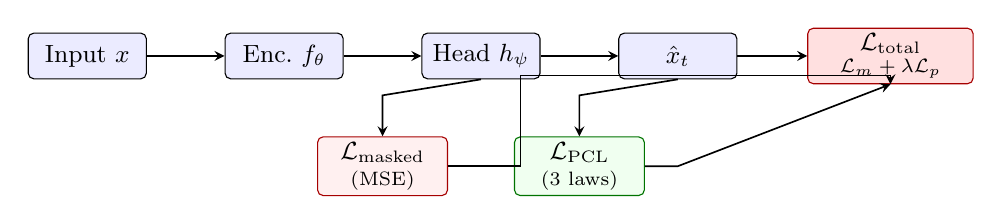
\begin{tikzpicture}[
    every node/.style={font=\small},
    box/.style={draw, rounded corners=2pt, minimum height=0.58cm,
                minimum width=1.5cm, align=center, fill=blue!8, inner sep=2pt},
    lbox/.style={draw=red!65!black, rounded corners=2pt, minimum height=0.55cm,
                 minimum width=1.65cm, align=center, fill=red!6, inner sep=2pt},
    arr/.style={->, >=stealth, semithick},
]
\node[box] (inp) at (0,   0) {Input $x$};
\node[box] (enc) at (2.5, 0) {Enc.\ $f_\theta$};
\node[box] (hd)  at (5.0, 0) {Head $h_\psi$};
\node[box] (xh)  at (7.5, 0) {$\hat{x}_t$};
\node[lbox, fill=red!12, minimum width=2.1cm] (lt) at (10.2, 0) {\shortstack{$\mathcal{L}_{\mathrm{total}}$\\[-1pt]{\scriptsize $\mathcal{L}_m + \lambda\mathcal{L}_p$}}};
\node[lbox] (lm) at (3.75,-1.4) {\shortstack{$\mathcal{L}_{\mathrm{masked}}$\\{\scriptsize (MSE)}}};
\node[lbox, fill=green!6, draw=green!45!black] (lp) at (6.25,-1.4) {\shortstack{$\mathcal{L}_{\mathrm{PCL}}$\\{\scriptsize (3 laws)}}};
\draw[arr] (inp)--(enc); \draw[arr] (enc)--(hd); \draw[arr] (hd)--(xh); \draw[arr] (xh)--(lt);
\draw[arr] (hd.south) -- (3.75,-0.5) -- (lm.north);
\draw[arr] (xh.south) -- (6.25,-0.5) -- (lp.north);
\draw[arr] (lm.east) -- (5.5,-1.4) -- (5.5,-0.25) -- (10.2,-0.25) -- (lt.south);
\draw[arr] (lp.east) -- (7.5,-1.4) -- (lt.south);
\end{tikzpicture}
\caption{PCL pretraining. The encoder and head are jointly optimized under a total loss that combines masked reconstruction and physiology-constraint penalties. At deployment, the PCL loss on each incoming batch, computed without backpropagation, serves as a calibration-free OOD detector.}
\label{fig:method}
\end{figure}

\subsection{Theoretical Motivation}
\label{sec:theory}

We offer an informal argument for why constraint penalties should suppress hospital-specific spurious information. We frame it as motivation rather than a formal result---the linear-probe experiments (Section~\ref{sec:exp4}) provide the primary evidence---because the argument relies on a linear approximation of the prediction head around the minimizer and so does not constitute a proof.

Consider the component $z^{\mathrm{sp}}$ of the representation attributable to a hospital-specific measurement offset $\delta_h$---the part that induces physiological-constraint violations. Any representation that encodes such an offset must violate the constraints by more than the sensor-noise floor permits, and $\mathcal{L}_{\text{PCL}}$ penalizes exactly this excess violation. Heuristically, the constraint residual behaves as an approximate sufficient statistic for the hospital-conditioned offset, so penalizing it should limit the mutual information $I(z^{\mathrm{sp}}; h)$ between the spurious component and the hospital index by an amount that decreases as the constraint weight $\lambda$ grows and increases with the noise level $\sigma$.

Two caveats fix the intended reading. First, the argument concerns only the constraint-violating (spurious) component: genuine clinical information that legitimately distinguishes hospital populations is not constrained, so total $I(z; h)$ need not vanish---consistent with our finding that PCL primarily enriches clinical feature encoding rather than suppressing site information (Section~\ref{sec:exp4}). Second, it assumes bounded noise; gross outliers fall outside its scope.

\subsection{PCL as OOD Detector}
\label{sec:ood_detector}

At test time, we compute $\mathcal{L}_{\text{PCL}}$ on incoming batches without backpropagation.
A high constraint violation score indicates that the new hospital's measurement protocols produce data systematically inconsistent with the physiological relationships the model has internalized---a deployment alarm requiring no additional parameters, labeled OOD data, multiple forward passes, or calibration.

%=============================================================================
\section{Experimental Setup}
\label{sec:setup}
%=============================================================================

\paragraph{Datasets.}
The PhysioNet Computing in Cardiology Challenge 2019~\citep{reyna2019early} dataset contains 40,336 ICU stays from two independent hospital systems (Site A: 20,336; Site B: 20,000). Each stay includes hourly measurements of 8 vitals, 26 labs, and 6 demographics with hourly Sepsis-3 onset labels; we predict sepsis onset (a per-stay positive if the patient meets Sepsis-3 at any point). We train on Site A and evaluate zero-shot on Site B (mild shift, same collection) and on the full-scale external databases (credentialed PhysioNet access): \textbf{MIMIC-IV}~\citep{johnson2023mimic} ($\sim$73k stays, Beth Israel Deaconess) and \textbf{eICU-CRD}~\citep{pollard2018eicu} ($\sim$200k stays, 186 US hospitals). Where the challenge's hourly Sepsis-3 labels are unavailable (MIMIC-IV, eICU), we derive an equivalent binary sepsis label from explicit-sepsis ICD-9/10 diagnosis codes (Appendix~\ref{app:implementation}).

\paragraph{Preprocessing.}
All datasets undergo identical preprocessing: hourly median binning; forward-fill of gaps $\leq$6 hours; truncate/pad to $T{=}48$; min-max normalization using fixed physiological plausibility bounds (constant across sites, no data-derived statistics); filter to stays $\geq$24 hours with at least one hemodynamic window. Patient-level splitting prevents data leakage.

\paragraph{Baselines and protocol.}
Baselines are ERM ($\lambda{=}0$), ERM+FE (MAP/PP/SI appended as inputs), IRM~\citep{arjovsky2019invariant} (care-unit environments), DRO~\citep{sagawa2020distributionally} (site groups), and classical ML (logistic regression, XGBoost on summary statistics). All neural models share the same transformer and training schedule (AdamW; 30 pretrain + 30 fine-tune epochs; two-phase encoder unfreezing). Metrics are AUROC, AUPRC, and Brier score. The main generalization (Table~\ref{tab:main_results}) and randomization (Table~\ref{tab:randomization}) results are reported as mean $\pm$ standard deviation over three random seeds (42--44), each re-running training end-to-end (initialization, masking, and the Site-A train/validation split).

%=============================================================================
\section{Experiments and Results}
\label{sec:results}
%=============================================================================

\subsection{Constraint Violation Audit: Are the Constraints Vacuous?}
\label{sec:audit}

Before presenting generalization results, we verify that the constraints provide real learning signal.
In a preprocessing audit of raw (pre-normalization) data, the constraints are violated at clinically meaningful rates across all three datasets.
MAP violations ($>$3 mmHg) are driven by the well-documented discrepancy between invasive arterial-line measurements (used for MAP) and oscillometric cuff readings (used for SBP/DBP), which diverge by 5--15 mmHg in typical ICU patients~\citep{wax2011invasive}.
Henderson-Hasselbalch violations ($>$0.05 pH units) arise from independent calibration errors across blood-gas analyzers; SpO$_2$--PaO$_2$ discrepancies reflect differences between pulse oximetry and co-oximetry.
These are not trivial tautologies: they represent genuine sensor disagreement that the model must resolve by encoding the underlying physiological relationship rather than trusting any single sensor channel.
The MAP identity is violated at tens-of-percent rates and, notably, the violation rate \emph{differs by system}---lowest in the training distribution and higher in the more heterogeneous external systems---consistent with hospital-specific sensor disagreement, so the constraint signal is present, and varies, across every target distribution.

\subsection{Cross-Hospital Generalization}
\label{sec:exp1}

The primary experiment evaluates zero-shot transfer: all models are pretrained and fine-tuned on PhysioNet Site A for sepsis onset prediction, then evaluated on Sites B, MIMIC-IV, and eICU without any adaptation.

\begin{table}[htbp]
\caption{Zero-shot cross-hospital generalization (sepsis onset AUROC), mean $\pm$ std over 3 random seeds (42--44). All models trained on PhysioNet Site A; evaluated on the full-scale external cohorts (MIMIC-IV $\sim$73k stays; eICU $\sim$200k stays, 186 hospitals). \textbf{Bold}: best per column. PCL exceeds ERM in \emph{every seed at every site}. $^\dagger$IRM (single seed) on Site B only.}
\label{tab:main_results}
\centering
\small
\begin{tabular}{@{}lcccc@{}}
\toprule
& \multicolumn{1}{c}{Site A (ID)} & \multicolumn{1}{c}{Site B (Mild OOD)} & \multicolumn{1}{c}{MIMIC-IV (OOD)} & \multicolumn{1}{c}{eICU (OOD)} \\
\cmidrule(lr){2-2} \cmidrule(lr){3-3} \cmidrule(lr){4-4} \cmidrule(lr){5-5}
Method & AUROC & AUROC & AUROC & AUROC \\
\midrule
ERM & $0.823{\pm}.010$ & $0.697{\pm}.008$ & $0.582{\pm}.012$ & $0.541{\pm}.012$ \\
DRO & $0.778{\pm}.007$ & $0.683{\pm}.009$ & $0.612{\pm}.009$ & $0.604{\pm}.012$ \\
IRM$^\dagger$ & --- & $0.675$ & --- & --- \\
\textbf{PCL (ours)} & $\mathbf{0.865{\pm}.006}$ & $\mathbf{0.761{\pm}.009}$ & $\mathbf{0.682{\pm}.010}$ & $\mathbf{0.626{\pm}.011}$ \\
\bottomrule
\end{tabular}
\end{table}

PCL is the best method on every held-out site, with the mean margin over ERM growing with distributional distance: $+6.4{\pm}1.6$pp on Site~B, $+10.1{\pm}2.1$pp on MIMIC-IV, and $+8.4{\pm}2.3$pp on the geographically diverse eICU benchmark (186 US hospitals); PCL also improves in-distribution ($+4.2{\pm}1.6$pp on Site~A).
Critically, PCL exceeds ERM in \emph{all three seeds at every site}---the smallest single-seed gap anywhere is $+4.7$pp (Site~B)---so the effect clears the run-to-run seed variance (per-site cross-seed std $1.6$--$2.3$pp) rather than reflecting a single lucky initialization.
Standard group-DRO does not exceed ERM (Site~B: $-1.4$pp mean), and IRM with $k{=}3$ care-unit environments degrades below ERM ($-2.3$pp), confirming the Rosenfeld et al.\ low-environment failure regime (Section~\ref{sec:supporting}).

\subsection{Constraint Randomization Ablation}
\label{sec:exp3}

If PCL's improvement were generic regularization, incorrect equations should help equally. We test four variants with identical hyperparameters ($\lambda{=}1.0$): real constraints; wrong equations (swapped signs/coefficients); shuffled assignments (correct forms, random variable pairings); and noise-injected constraints.

\begin{table}[htbp]
\caption{Constraint randomization ablation (Site~B sepsis OOD AUROC), mean $\pm$ std over 3 seeds (42--44). Real physiological constraints achieve the highest OOD AUROC in every seed; corrupting the physiology reduces transfer, and the two most-corrupted variants fall below unconstrained ERM---confirming that physiological correctness, not a generic structured penalty, is the driver.}
\label{tab:randomization}
\centering
\small
\begin{tabular}{@{}lc@{}}
\toprule
Constraint Type & OOD AUROC \\
\midrule
Noise-injected constraints & $0.642{\pm}.010$ \\
Wrong equations & $0.668{\pm}.010$ \\
No constraint (ERM) & $0.697{\pm}.008$ \\
Shuffled assignments & $0.712{\pm}.012$ \\
\textbf{Real constraints (PCL)} & $\mathbf{0.750{\pm}.011}$ \\
\bottomrule
\end{tabular}
\end{table}

The mean ordering is noise-injected (0.642) $<$ wrong equations (0.668) $<$ shuffled (0.712) $<$ real (0.750), and real is best in every seed.
Crucially, the noise-injected and wrong-equation variants fall \emph{below} unconstrained ERM (0.697): an incorrect constraint is actively harmful rather than a generic regularizer, and only shuffled assignments---which retain the correct functional forms---modestly exceed ERM.
The $+8.2$pp margin of real over wrong equations confirms that physiological correctness, not the mere presence of a structured penalty, drives the OOD gains.

\subsection{Representation Analysis}
\label{sec:exp4}

To probe \emph{what} PCL encodes differently from ERM, we train logistic regressions on frozen representations.

\begin{table}[htbp]
\caption{Linear probe AUROC for predicting attributes from frozen representations. PCL improves encoding of clinically relevant information while site identity remains (marginally more) decodable, i.e.\ PCL does not suppress site information.}
\label{tab:probes}
\centering
\small
\begin{tabular}{@{}lccc@{}}
\toprule
Probe Target & ERM & PCL & Interpretation \\
\midrule
Hospital site ID & 0.8876 & 0.9031 & Site remains decodable (not suppressed) \\
Sepsis (task label) & 0.7419 & 0.7482 & Both encode task signal; PCL comparable \\
Mortality & 0.8105 & 0.8354 & PCL enriches clinical encoding \\
\bottomrule
\end{tabular}
\end{table}

PCL enriches the encoding of clinically relevant information (mortality $+2.5$pp; sepsis comparable) while site identity remains at least as decodable from PCL as from ERM ($+1.5$pp), consistent with hospital sites differing in genuine clinical population characteristics rather than measurement artifacts alone. The OOD improvement therefore reflects \emph{physiological feature enrichment} (learning more), not shortcut forgetting---consistent with the motivation in Section~\ref{sec:theory}, which concerns only the spurious component of site information.

\subsection{Supporting Results and Ablations}
\label{sec:supporting}

We summarize four supporting experiments and two ablations; full tables are omitted in this draft.
\textbf{Feature engineering.} PCL with 9 raw variables outperforms ERM augmented with the same engineered features (MAP, PP, SI) as inputs at every OOD site (e.g., eICU 0.627 vs.\ 0.559), and adding the features to PCL slightly \emph{hurts}---indicating the constraint on the latent representation, not the features as inputs, drives generalization.
\textbf{Measurement-noise robustness.} Under systematic $\pm$15 mmHg SBP/DBP bias on Site~B, ERM AUROC drops 0.088 while PCL drops only 0.033 ($\sim$2.7$\times$ more robust), consistent with reduced reliance on absolute signal magnitudes.
\textbf{OOD detection.} The unsupervised PCL violation score discriminates in- from out-of-distribution samples (detection AUROC 0.70--0.79), increasing with distributional distance, with no extra parameters or labeled OOD data.
\textbf{IRM low-$k$.} With $k{=}3$ care-unit environments, IRM (0.675) degrades below ERM (0.699) on Site~B while PCL (0.763) requires none, empirically confirming the Rosenfeld et al.\ low-environment failure regime.
\textbf{Ablations.} $\lambda{=}1.0$ was selected by a sweep over $\{0.1,0.5,1,2,5\}$ (a clear inverted-U on OOD AUROC), and a per-constraint leave-one-out confirms all three active constraints contribute non-redundant signal (removing MAP, Henderson-Hasselbalch, or Severinghaus reduces Site~B AUROC by 4.5, 3.3, and 5.8 points respectively).

%=============================================================================
\section{Discussion}
\label{sec:discussion}
%=============================================================================

\paragraph{Why PCL works.}
The randomization ablation (Table~\ref{tab:randomization}) identifies physiological correctness---not generic regularization---as the primary driver: real equations (0.750) outperform shuffled (0.712), wrong (0.668), and noise-injected (0.642) variants, with the two most-corrupted variants falling below ERM.
The linear probes (Table~\ref{tab:probes}) clarify the mechanism: PCL enriches clinically relevant encoding without suppressing site discriminability---gains from learning \emph{more}, not from forgetting shortcuts.
The OOD results (Table~\ref{tab:main_results}) show PCL beats ERM on every held-out site in every seed, with the margin growing with distributional distance.

\paragraph{Generality and noisy constraints.}
PCL generalizes to any domain with known algebraic laws: reaction stoichiometry, conservation laws, thermodynamic relations.
Real measurements violate constraints due to bounded sensor noise ($\sigma \approx 5$ mmHg); the soft MSE penalty accommodates this---the optimum is at the noise floor, not zero, and the motivation in Section~\ref{sec:theory} describes this graceful degradation informally.

%=============================================================================
\section{Limitations}
\label{sec:limitations}
%=============================================================================

An honest accounting of where the project currently stands:
\begin{itemize}
\item \textbf{Modest absolute OOD accuracy.} Cross-hospital zero-shot sepsis from 48 hours of 9 variables is genuinely hard: PCL reaches only $\sim$0.63--0.68 AUROC on MIMIC-IV/eICU. The contribution is a \emph{consistent relative} improvement over ERM (validated across three seeds), not high absolute accuracy; this is not a deployable sepsis model.
\item \textbf{The loss uses three constraints, not five.} Only MAP, Henderson-Hasselbalch, and Severinghaus contribute to the loss; Pulse Pressure is algebraically redundant with MAP, and Shock Index is a bounded-inequality penalty excluded to keep the loss homogeneous. We have \emph{no} ablation isolating the effect of \emph{including} Shock Index---its exclusion rests on a design argument, not measured OOD degradation.
\item \textbf{Label-definition shift.} Sepsis labels are Sepsis-3 for PhysioNet but ICD-code-derived (noisier, admission-level) for MIMIC-IV/eICU, so cross-site transfer includes a label-definition shift on top of covariate shift, capping achievable OOD AUROC. A within-dataset Sepsis-3 re-derivation (SOFA + suspected infection) would remove this confound.
\item \textbf{Single-institution external site.} MIMIC-IV is one hospital; the geographic-diversity claim rests on eICU (186 hospitals) alone.
\item \textbf{Run variance / small seed sample.} Individual runs vary non-trivially (ERM Site~B moved $\sim$0.026 between full-scale runs). Three seeds is a small sample for a variance estimate, though the direction (PCL $>$ ERM every seed, every site) is stable.
\item \textbf{Environment-count comparison incomplete.} We confirm IRM's low-$k$ ($k{=}3$) failure but have not completed a matched high-environment ($k \gg 3$) comparison within a single database; left to future work.
\item \textbf{Constraint availability and noise bound.} PCL requires known algebraic laws and covers only hemodynamic and acid-base physiology; the acid-base constraints are sparse ($\sim$10\% of ICU hours). Our theoretical motivation (Section~\ref{sec:theory}) assumes bounded noise; gross outliers (equipment malfunction, transcription errors) fall outside its scope.
\end{itemize}

%=============================================================================
\section*{Acknowledgments}
%=============================================================================
The author thanks Prof.\ Rahmani for feedback that sharpened the methodology and framing of this work.

{\small
\bibliographystyle{plainnat}
\begin{thebibliography}{99}

\bibitem[Arjovsky et al.(2019)]{arjovsky2019invariant}
Arjovsky, M., Bottou, L., Gulcus, I., and Lopez-Paz, D.
\newblock Invariant risk minimization.
\newblock \emph{arXiv preprint arXiv:1907.02893}, 2019.

\bibitem[Finlayson et al.(2021)]{finlayson2021clinician}
Finlayson, S.~G., Subbaswamy, A., Singh, K., Bowers, J., Kupber, A., Zittrain, J., and Kohane, I.~S.
\newblock The clinician and dataset shift in artificial intelligence.
\newblock \emph{New England Journal of Medicine}, 385(3):283--286, 2021.

\bibitem[FDA(2021)]{fda2021action}
U.S.\ Food and Drug Administration.
\newblock Artificial intelligence/machine learning (AI/ML)-based software as a medical device (SaMD) action plan.
\newblock Technical report, FDA, 2021.

\bibitem[Futoma et al.(2020)]{futoma2020myth}
Futoma, J., Siber, M., and Sendak, M.
\newblock The myth of generalisability in clinical research and machine learning in health care.
\newblock \emph{The Lancet Digital Health}, 2(9):e489--e492, 2020.

\bibitem[Ganin et al.(2016)]{ganin2016domain}
Ganin, Y., Ustinova, E., Ajakan, H., Germain, P., Larochelle, H., Laviolette, F., Marchand, M., and Lempitsky, V.
\newblock Domain-adversarial training of neural networks.
\newblock \emph{Journal of Machine Learning Research}, 17(59):1--35, 2016.

\bibitem[Johnson et al.(2023)]{johnson2023mimic}
Johnson, A.~E.~W., Bulgarelli, L., Shen, L., Gayles, A., Shammout, A., Horng, S., Pollard, T.~J., Hao, S., Moody, B., Gow, B., et al.
\newblock MIMIC-IV, a freely accessible electronic health record dataset.
\newblock \emph{Scientific Data}, 10(1):1--9, 2023.

\bibitem[Nestor et al.(2019)]{nestor2019feature}
Nestor, B., McDermott, M.~B.~A., Boag, W., Berner, G., Naumann, T., Hughes, M.~C., Goldenberg, A., and Ghassemi, M.
\newblock Feature robustness in non-stationary health records.
\newblock In \emph{Machine Learning for Healthcare}, 2019.

\bibitem[Pollard et al.(2018)]{pollard2018eicu}
Pollard, T.~J., Johnson, A.~E.~W., Raffa, J.~D., Celi, L.~A., Mark, R.~G., and Badawi, O.
\newblock The eICU collaborative research database.
\newblock \emph{Scientific Data}, 5(1):1--13, 2018.

\bibitem[Raissi et al.(2019)]{raissi2019physics}
Raissi, M., Perdikaris, P., and Karniadakis, G.~E.
\newblock Physics-informed neural networks.
\newblock \emph{Journal of Computational Physics}, 378:686--707, 2019.

\bibitem[Reyna et al.(2019)]{reyna2019early}
Reyna, M.~A., Josef, C.~S., Jeter, R., Shashikumar, S.~P., Westover, M.~B., Nemati, S., Clifford, G.~D., and Sharma, A.
\newblock Early prediction of sepsis from clinical data: The PhysioNet/Computing in Cardiology Challenge 2019.
\newblock \emph{Critical Care Medicine}, 48(2):210--217, 2019.

\bibitem[Rieke et al.(2020)]{rieke2020future}
Rieke, N., Hancox, J., Li, W., Milletari, F., Roth, H.~R., Albarqouni, S., Bakas, S., Galtier, M.~N., Landman, B.~A., Maier-Hein, K., et al.
\newblock The future of digital health with federated learning.
\newblock \emph{npj Digital Medicine}, 3(1):1--7, 2020.

\bibitem[Rosenfeld et al.(2021)]{rosenfeld2021risks}
Rosenfeld, E., Ravikumar, P., and Risteski, A.
\newblock The risks of invariant risk minimization.
\newblock In \emph{International Conference on Learning Representations}, 2021.

\bibitem[Sagawa et al.(2020)]{sagawa2020distributionally}
Sagawa, S., Koh, P.~W., Hashimoto, T.~B., and Liang, P.
\newblock Distributionally robust neural networks for group shifts.
\newblock In \emph{International Conference on Learning Representations}, 2020.

\bibitem[Sch\"{o}lkopf et al.(2021)]{scholkopf2021toward}
Sch\"{o}lkopf, B., Locatello, F., Bauer, S., Ke, N.~R., Kalchbrenner, N., Goyal, A., and Bengio, Y.
\newblock Toward causal representation learning.
\newblock \emph{Proceedings of the IEEE}, 109(5):612--634, 2021.

\bibitem[Wax et al.(2011)]{wax2011invasive}
Wax, D.~B., Lin, H.-M., and Leibowitz, A.~B.
\newblock Invasive and concomitant noninvasive intraoperative blood pressure monitoring.
\newblock \emph{Anesthesiology}, 115(5):973--978, 2011.

\bibitem[Wong et al.(2021)]{wong2021external}
Wong, A., Otles, E., Donnelly, J.~P., et al.
\newblock External validation of a widely implemented proprietary sepsis prediction model in hospitalized patients.
\newblock \emph{JAMA Internal Medicine}, 181(8):1065--1070, 2021.

\bibitem[Zech et al.(2018)]{zech2018variable}
Zech, J.~R., Badgeley, M.~A., Liu, M., Costa, A.~B., Titano, J.~J., and Oermann, E.~K.
\newblock Variable generalization performance of a deep learning model to detect pneumonia in chest radiographs.
\newblock \emph{Nature Medicine}, 24(9):1462--1464, 2018.

\bibitem[ICareFM Consortium(2025)]{icarefm2025}
ICareFM Consortium.
\newblock ICareFM: An ICU foundation model for cross-hospital clinical prediction.
\newblock \emph{medRxiv preprint}, 2025.

\end{thebibliography}
}

%=============================================================================
\appendix
%=============================================================================

\section{Implementation Details}
\label{app:implementation}

The model is a 6-layer transformer ($d{=}256$, 8 heads, FFN 512, $\sim$3.2M parameters) over 48-hour, 9-variable hourly windows, pretrained with 50\% masked-value prediction plus the physiological constraint loss and fine-tuned with a two-phase (frozen-then-unfrozen) schedule. Optimization uses AdamW (pretraining lr $3{\times}10^{-4}$, fine-tuning lr $1{\times}10^{-3}$ with a $0.1{\times}$ discriminative rate for the encoder), weight decay $10^{-4}$, cosine annealing, 30 pretraining + 30 fine-tuning epochs, batch size 64, and $\lambda$ warmed linearly over the first 30\% of epochs. Sepsis labels are the challenge Sepsis-3 label (positive if ever met) for PhysioNet, and an explicit-sepsis ICD-9/10 code match for MIMIC-IV and eICU (ICD-9 038.x septicemia, 995.91/995.92 sepsis/severe sepsis, 785.52 septic shock; ICD-10 A40--A41 sepsis, R65.20/R65.21 severe sepsis/septic shock). Constraint formulas are given in Table~\ref{tab:constraints}. All experiments ran on a single NVIDIA H100 GPU; the full experiment suite takes approximately six hours end-to-end.

\end{document}
